
\section{态射的像：谢瓦莱定理与消元理论}

在本节中，我们要回答一个问题——早在听到「代数几何」这个词之前，你恐怕就琢磨过它了。如果你手头有一批带不定系数的多元多项式方程，你自然会问：系数满足什么条件，（公共）解才存在。鉴于问题本质是代数的，你有理由指望答案也纯属代数——它不该是「随机」的，也不该掺进指数函数、余弦之类古怪的函数。你应当期望答案由「代数条件」给出。事实确实如此，而且这件事可以卓有成效地改述为簇或概形之映射的像的问题；换了这副面孔，它便由谢瓦莱定理~8.4.2 给出解答（更精细的证明见\S8.4.8）。作为推论，我们还顺带得到\trNullstellensatz（\cref{thm:hilbert-nullstellensatz}）的一个立竿见影的证明（\S8.4.3）。

在某些情形，像还要更漂亮。例如，有限态射的像总是闭的（\mbox{练习~8.3.L}）。我们将证明一条经典结果——\trFundamentalTheoremOfEliminationTheory{}（Fundamental Theorem of Elimination Theory）~8.4.10，它本质上把这条事实推广（如\S9.3.5 所解释的）到从射影空间出发的映射。

沿另一个方向，我们将看到：在某些好的境况下（「平坦」再多一点点；见\mbox{练习~24.5.G}），态射是开的（开子集的像是开的）；一个例子（你可以试着直接证明）便是 $\mathbb{A}^1_B\to\Spec B$。

\textbf{8.4.1.\ \trChevalley{}定理。}

若 $\pi\colon X\to Y$ 是概形间的态射，则把 $\pi$ 的像当\emph{集合}看，其含义是清楚的：取 $Y$ 中那些身为 $X$ 中点之像的点即可。我们知道，像可以是开的（开嵌入），也见过像是闭的情形，以及更一般地，局部闭（locally closed）的情形。
但它还可以更怪：考虑由 $(x,y)\mapsto(x,xy)$ 给出的态射 $\mathbb{A}^2_k\to\mathbb{A}^2_k$。其像是全平面挖去 $y$-轴、再把原点放回来（图~\ref{fig:constructible-image-xy}）。我们为此现象下一个定义。\trNoetherian\trTopologicalSpace{}的一个子集称为\textbf{\trConstructible{}子集}（constructible subset），如果它属于由子集组成的、满足下列三条的最小族：(i) 每个开集都在族中；(ii) 族中成员的有限交仍在族中；(iii) 族中成员的补集也在族中。例如，$(x,y)\mapsto(x,xy)$ 的像是\trConstructible{}的。


\begin{figure}[htbp]
\centering
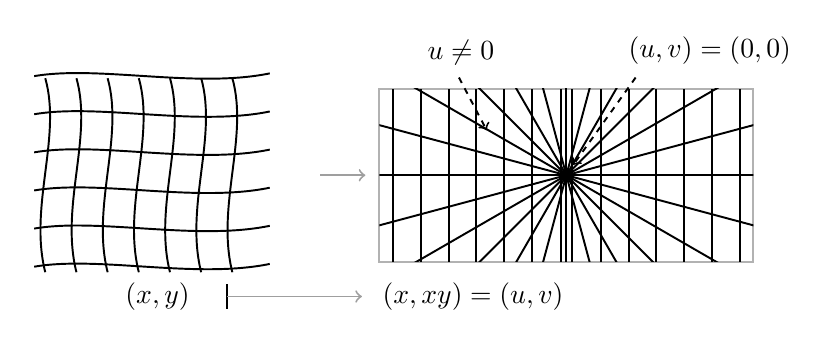
\begin{tikzpicture}[scale=0.88,line width=0.7pt]
  \begin{scope}[shift={(-5.9,1.25)}]
    \foreach \i in {0,...,6}
      \draw ({-1.62+0.45*\i},-1.4)
            .. controls ({-1.86+0.45*\i},-0.45) and ({-1.38+0.45*\i},0.55) ..
            ({-1.62+0.45*\i},1.4);
    \foreach \j in {0,...,5}
      \draw (-1.78,{-1.32+0.55*\j})
            .. controls (-0.85,{-1.16+0.55*\j}) and (0.55,{-1.5+0.55*\j}) ..
            (1.62,{-1.28+0.55*\j});
  \end{scope}
  \draw[gray!75,->] (-3.55,1.25) -- (-2.9,1.25);
  \draw[gray!60] (-2.7,0) rectangle (2.7,2.5);
  \begin{scope}
    \clip (-2.7,0) rectangle (2.7,2.5);
    \foreach \a in {0,15,...,345}
      \draw ({3.6*cos(\a)},{1.25+3.6*sin(\a)}) -- (0,1.25);
    \foreach \x in {-2.5,-2.1,...,-0.5} \draw (\x,0) -- (\x,2.5);
    \foreach \x in {0.5,0.9,...,2.5} \draw (\x,0) -- (\x,2.5);
    \draw (-0.08,0) -- (-0.08,2.5);
    \draw (0.08,0) -- (0.08,2.5);
  \end{scope}
  \fill (0,1.25) circle (1.7pt);
  \node[anchor=south west] at (-2.15,2.7) {$u\neq0$};
  \draw[dash pattern=on 2.2pt off 2.2pt,->] (-1.55,2.66) -- (-1.15,1.9);
  \node[anchor=south west] at (0.75,2.7) {$(u,v)=(0,0)$};
  \draw[dash pattern=on 2.2pt off 2.2pt,->] (1.0,2.66) -- (0.1,1.4);
  \node at (-5.9,-0.5) {$(x,y)$};
  \draw (-4.9,-0.32) -- (-4.9,-0.68);
  \draw[gray!75,->] (-4.9,-0.5) -- (-2.95,-0.5);
  \node[anchor=west] at (-2.8,-0.5) {$(x,xy)=(u,v)$};
\end{tikzpicture}
\caption{$(x,y)\mapsto(x,xy)=(u,v)$ 的像。（依原书手绘图重绘。）}\label{fig:constructible-image-xy}
\end{figure}

\begin{exercise}[练习：\trConstructible{}子集是\trLocally\trClosed{}子集的有限不交并]\label{ex:constructible-finite-disjoint-union}
回想：拓扑空间 $X$ 的一个子集称为\textbf{局部闭}（locally closed），如果它是一个开子集与一个闭子集的交。（等价地，它可以是闭子集的开子集，或者开子集的闭子集。日后要把这条推广到开子概形、闭子概形与\trLocally\trClosed{}子概形上去时，我们会遇到麻烦；见\mbox{练习~9.2.C}。）证明：诺特拓扑空间 $X$ 的一个子集是\trConstructible{}的，当且仅当它是\trLocally\trClosed{}子集的有限\trDisjointUnion。
\end{exercise}

作为推论，若 $X\to Y$ 是诺特拓扑空间之间的\trContinuousMap，则\trConstructible{}集的原像仍是\trConstructible{}集。（一条重要的评注：把「所论拓扑空间是诺特的」列为假设，唯一的原因是我们只在诺特的框架里定义了\trConstructible{}集。把可构造性（constructibility）这一概念推广到更一般的拓扑空间，见于\mbox{练习~10.3.I}。）

\begin{exercise}[容易的练习（用于\S8.4.3）]\label{ex:generic-point-not-constructible}
证明：$\mathbb{A}^1_k$ 的\trGenericPoint{}并不构成 $\mathbb{A}^1_k$ 的\trConstructible{}子集（其中 $k$ 是域）。
\end{exercise}

\begin{exercise}[练习（用于\mbox{练习~24.5.G}）]\label{ex:constructible-stable-specialization}
\begin{enumerate}[label=(\alph*)]
\item 证明：诺特概形的\trConstructible{}子集是闭的，当且仅当它在「\trSpecialization{}之下稳定」。更精确地：若 $Z$ 是诺特概形 $X$ 的\trConstructible{}子集，则 $Z$ 是闭的，当且仅当对每一对满足 $y_1\in\overline{y_2}$ 的点 $y_1$、$y_2$，只要 $y_2\in Z$，就有 $y_1\in Z$。「若」一方的提示：证明 $Z$ 能写成 $\coprod_{i=1}^{n}U_i\cap Z_i$，其中诸 $U_i\subset X$ 是开集，诸 $Z_i\subset X$ 是闭集。再证明：$Z$ 能写成 $\coprod_{i=1}^{n}U_i\cap Z_i$（其中的 $n$、$U_i$、$Z_i$ 尽可换作别的），使得每个 $Z_i$ 都\trIrreducible{}且与 $U_i$ 相交。然后用「\trSpecialization{}之下稳定」与诸 $Z_i$ 的\trGenericPoint{}证明：对一切 $i$ 都有 $Z_i\subset Z$，从而 $Z=\cup Z_i$。
\item 证明：诺特概形的\trConstructible{}子集是开的，当且仅当它在「\trGenerization{}之下稳定」。（提示：由 (a) 一行即得。）
\end{enumerate}
\end{exercise}

概形态射的像可以比\trConstructible{}集还要怪异。事实上，设 $S$ 是概形 $Y$ 的\emph{任意}子集，它都能充当某个态射的像：令 $X$ 为 $S$ 的全部点的剩余域之谱的\trDisjointUnion，令 $\pi\colon X\to Y$ 为自然映射。这相当病态；但在任何合理的情势下，像都不会比前例 $(x,y)\mapsto(x,xy)$ 中的像本质上更坏。谢瓦莱定理把这件事说得一清二楚。

\textbf{8.4.2.\ \trChevalley{}定理。}\ ——\ \emph{若 $\pi\colon X\to Y$ 是\trNoetherian\trScheme{}间的\trFiniteType\trMorphism，则任何\trConstructible{}集的像都可构造。特别地，$\pi$ 的像是\trConstructible{}的。}

（若你恰是会在意此事的少数派：向局部有限表现态射的推广，见\S10.3.8。）我们先给出几条或许出人意料的重要推论，再来讨论证明；出人意料之处在于，它们竟是一条看似十足几何、十足拓扑的定理的代数推论。第一条便是\trNullstellensatz{}的一个证明。

\textbf{8.4.3.}\ \emph{\trNullstellensatz（\cref{thm:hilbert-nullstellensatz}）的证明。}\quad 我们要证明：若 $K$ 是 $k$ 的\trFieldExtension{}且作为 $k$-\trAlgebra{}有限生成，比如说由 $x_1,\dots,x_n$ 生成，则它是域的\trFiniteFieldExtension。只需证明每个 $x_i$ 在 $k$ 上都是\trAlgebraic{}的。但若有某个 $x_i$ 在 $k$ 上不是\trAlgebraic{}的，我们便有一个环的包含映射 $k[x_i]\hookrightarrow K$，它对应于\trFiniteType{} $k$-\trScheme{}之间的一个\trDominant\trMorphism{} $\pi\colon\Spec K\to\mathbb{A}^1_k$。当然，$\Spec K$ 是单独一个点，故 $\pi$ 的像仅有一点。由谢瓦莱定理~8.4.2 与\cref{ex:generic-point-not-constructible}，$\pi$ 的像不是 $\mathbb{A}^1_k$ 的\trGenericPoint，于是 $\im(\pi)$ 是 $\mathbb{A}^1_k$ 的一个\trClosedPoint，从而 $\pi$ 不\trDominant。\hfill$\square$

同样的想法可用于下面的练习。

\begin{exercise}[练习（到域的\trQuasifinite{}态射皆有限）]\label{ex:quasifinite-to-field-finite}
设 $\pi\colon X\to\Spec k$ 是\trQuasifinite{}（quasifinite）态射。
证明：$\pi$ 是有限的。（提示：先处理仿射情形 $X=\Spec A$，其中 $A$ 在 $k$ 上有限生成。假设 $A$ 含有一个在 $k$ 上不\trAlgebraic{}的元素 $x$，也就是说，我们有一个包含映射 $k[x]\hookrightarrow A$。\mbox{练习~8.3.G} 或许可派上用场。）
\end{exercise}

\begin{exercise}\label{ex:finite-type-over-z-finite-residue}
设 $X$ 是 $\Spec\mathbb{Z}$ 上\trFiniteType{}的概形，而 $p$ 是 $X$ 的一个\trClosedPoint。证明：\trResidueField{} $\kappa(p)$ 是有限域。
\end{exercise}

\begin{exercise}[练习（对簇的映射，满性可在闭点上检验）]\label{ex:surjectivity-closed-points}
假设谢瓦莱定理~8.4.2。证明：仿射 $k$-簇之间的态射 $\pi\colon X\to Y$ 是满的，当且仅当它在闭点上是满的（即：$Y$ 的每个\trClosedPoint{}都是 $X$ 的某个\trClosedPoint{}的像）。（等到在定义~11.2.9 中一般地定义了簇之后，你会看到：你的论证无须改动便可照搬，只需抹去「仿射」这个形容词。）
\end{exercise}

\textbf{8.4.4.\ \trChevalley{}定理~8.4.2 的证明。}

\begin{exercise}\label{ex:chevalley-reduction}
\begin{enumerate}[label=(\alph*)]
\item 把谢瓦莱定理的证明化归到 $Y$ 为\trAffine{}的情形，比如说 $Y=\Spec B$。
\item 进一步化归到 $X$ 为\trAffine{}的情形，比如说 $X=\Spec B[t_1,\dots,t_n]/I$。
\item 进一步化归到 $X=\mathbb{A}^n_B=\Spec B[t_1,\dots,t_n]$ 的情形。
\item 进一步化归到 $X=\mathbb{A}^1_B=\Spec B[t]$ 的情形。
\end{enumerate}
\end{exercise}

至此，任务已化简为：给定 $\pi\colon X=\Spec B[t]\to\Spec B=Y$，证明 $X$ 的任何\trConstructible{}子集在 $Y$ 中的像可构造。由于\trConstructible{}集是\trLocally\trClosed{}子集的有限并（\cref{ex:constructible-finite-disjoint-union}——我们正处在诺特的情势中），只需证明：$X$ 的任何\emph{局部闭}子集 $Z$ 在 $Y$ 中的像可构造。

\textbf{8.4.5.}\ \emph{一个重要的特殊情形。}\quad 我们从 $Z$ 是 $X=\mathbb{A}^1_B$ 的\emph{闭}子集的情形入手，比如说
\[
Z=V(f_1(t),\dots,f_r(t))\text{，}\qquad\text{其中}\quad
f_i(t)=a_{id_i}t^{d_i}+\cdots+a_{i1}t+a_{i0}\text{，}
\]
诸 $a_{ij}\in B$，于是 $f_i(t)\in B[t]$，而 $d_i=\deg f_i(t)$。

现在 $Y=\Spec B$ 是诸\trLocally\trClosed{}子集 $Y_{\vec{e}}$ 的有限\trDisjointUnion，后者由 $\vec{e}=(e_1,\dots,e_r)$ 标号，其中 $e_i\in\mathbb{Z}$，$-1\le e_i\le d_i$；$Y_{\vec{e}}$ 是 $f_1(t),\dots,f_r(t)$ 分别具有「\trTrueDegree{}」（true degree）$e_1,\dots,e_r$ 的\trLocus：$f_i(t)$ 中 $t^{e_i}$ 的系数非零，而「更高次」的系数为零（在 $Y_{\vec{e}}$ 的各点处）。更精确地说：$Y_{\vec{e}}\subset Y$ 是使 $a_{ie_i}\neq0$、且对 $j>e_i$ 有 $a_{ij}=0$ 的\trLocus。（按此约定，零多项式的「\trTrueDegree{}」为 $-1$。）还要更精确的话，我们定义 $Y_{\vec{e}}:=\Spec B_{\vec{e}}$，其中
\[
B_{\vec{e}}:=\frac{B_{\prod_i a_{ie_i}}}{\left(a_{ij}\right)_{j>e_i}}\text{，}\qquad\text{于是}\quad
Y_{\vec{e}}=\Bigl(\mathop{\cap}\limits_{i}D(a_{ie_i})\Bigr)\cap
\Biggl(\mathop{\cap}\limits_{i,\ j>e_i}V(a_{ij})\Biggr)\text{。}
\]
若 $\vec{e}=(-1,\dots,-1)$，则
\begin{equation*}\tag{8.4.5.1}\label{eq:true-degree-fibration}
\pi^{-1}(Y_{\vec{e}})\xrightarrow{\ \pi\ }Y_{\vec{e}}
\end{equation*}
是满的（映射 \eqref{eq:true-degree-fibration} 即 $\Spec B_{(-1,\dots,-1)}[t]\to\Spec B_{(-1,\dots,-1)}$）；而若 $\vec{e}\neq(-1,\dots,-1)$，则 \eqref{eq:true-degree-fibration} 是一个有限态射，对应的环映射为
\[
B_{\vec{e}}\longrightarrow B_{\vec{e}}[t]\Bigm/\Bigl(t^{e_1}+\tfrac{a_{1(e_1-1)}}{a_{1e_1}}t^{e_1-1}
+\cdots+\tfrac{a_{10}}{a_{1e_1}},\ \dots,\ t^{e_r}+\tfrac{a_{r(e_r-1)}}{a_{re_r}}t^{e_r-1}
+\cdots+\tfrac{a_{r0}}{a_{re_r}}\Bigr)\text{。}
\]
（右边的环作为 $B_{\vec{e}}$-\trModule{}由 $1,t,\dots,t^{\max(e_i)}$ 生成。）由于有限态射的像是闭的（\mbox{练习~8.3.L}），$\pi(Z)\cap Y_{\vec{e}}$（即 \eqref{eq:true-degree-fibration} 的像）是 $Y$ 的\trLocally\trClosed{}子集，故当 $Z$ 为闭时，$\pi(Z)$ 确实可构造。我们的重要特殊情形至此完成。

\textbf{8.4.6.}\ 注意，使整条\trFiber{} $\pi^{-1}(q)$ 都含于 $Z$ 内的那些点 $q\in Y$ 所构成的\trLocus，即 $\{\,q\in Y\ :\ \pi^{-1}(q)\subset Z\,\}$，是 $Y$ 的一个\emph{闭}子集：它就是 $\Spec B_{(-1,\dots,-1)}=\Spec B/(a_{ij})$。我们把它记作 $\mathrm{FL}(Z)\subset Y$，称为「$Z$ 的\trFiber\trLocus」，但只在本次证明的余下部分中使用。\footnote{译注：FL 系 fibral locus（\trFibralLocus{}）的首字母缩写。}

\textbf{8.4.7.}\ 最后，若 $Z$ 是\emph{局部闭}的，则 $\overline{Z}\subset X$ 是闭的，故 $\pi(\overline{Z})$ 是 $Y=\Spec B$ 的\trConstructible{}子集。定义 $\delta Z:=\overline{Z}\smallsetminus Z$，这是 $X$ 的一个闭子集；由\S8.4.6，$\mathrm{FL}(\overline{Z})$ 与 $\mathrm{FL}(\delta Z)$ 都是 $Y$ 的闭子集。既然 $\mathrm{FL}(\overline{Z})\smallsetminus\mathrm{FL}(\delta Z)$ 含于 $\pi(Z)$，而 $\mathrm{FL}(\delta Z)$ 含于 $\pi(Z)$ 的\trComplement，只需对开子集 $Y':=Y\smallsetminus(\mathrm{FL}(\overline{Z})\cup\mathrm{FL}(\delta Z))\subset Y$ 证明结果即可。令 $\pi'\colon X'=\mathbb{A}^1_{Y'}\to Y'$ 为 $\pi$ 在 $Y'$ 上方的限制，令 $Z'=Z\cap\mathbb{A}^1_{Y'}$（它在 $Y'$ 上方\trQuasifinite{}），并令 $\delta Z'=\overline{Z'}\smallsetminus Z'\subset\mathbb{A}^1_{Y'}$（其中 $\overline{Z'}$ 是 $Z'$ 在 $\mathbb{A}^1_{Y'}$ 中的\trClosure）。

\begin{exercise}\label{ex:delta-z-generic-fibers}
证明：闭子集 $\delta Z'\subset\mathbb{A}^1_{Y'}$ 与 $\pi'$ 的任何一般纤维都不相交，也就是说，与 $Y'$ 的任何\trGenericPoint{}的\trInverseImage{}不相交。进而证明：$Y'$ 有一片\trDense{}的开子集，与\trConstructible{}集 $\pi'(\delta Z')$ 不相交。
\end{exercise}

至此，我们已在 $\Spec B$ 的一片\trDense{}开子集之上证明了结果。

\begin{exercise}\label{ex:chevalley-noetherian-induction}
借助诺特归纳，以某种足够严格的方式收尾谢瓦莱定理~8.4.2 的证明。
\end{exercise}

\hfill$\square$

\textbf{8.4.8.}\ \hard\ \textbf{\trEliminationOfQuantifiers{}}（elimination of quantifiers）。\quad 在数不清的语境中都会冒出来的一类基本问题是：一个方程组何时有解。设想，比方说，你手头有一些系数在代数闭域 $\bar{k}$ 上、关于变量 $x_1,\dots,x_n$ 的多项式，你把其中一部分置为零，另一部分置为非零。（早在你认识任何概形理论之前，这个问题就有着根本上的趣味！）那么，系数上存在一条代数条件，它会告诉你解是否存在。以显而易见的方式在 $\bar{k}^n$ 上定义\trZariskiTopology：闭子集由方程切出。（这条的一个温和推广出现在\mbox{练习~12.2.L}中。）

\begin{exercise}[练习（代数闭域上的\trEliminationOfQuantifiers{}）]\label{ex:elimination-quantifiers}
取定代数闭域 $\bar{k}$。设已给定
\[
f_1,\dots,f_p,\ g_1,\dots,g_q\in\bar{k}[W_1,\dots,W_m,X_1,\dots,X_n]\text{。}
\]
证明：存在 $\bar{k}^m$ 的一个（\trZariski-）\trConstructible{}子集 $Y$，使得
\begin{equation*}\tag{8.4.8.1}\label{eq:elimination-equalities}
f_1(w_1,\dots,w_m,X_1,\dots,X_n)=\cdots=f_p(w_1,\dots,w_m,X_1,\dots,X_n)=0
\end{equation*}
且
\begin{equation*}\tag{8.4.8.2}\label{eq:elimination-inequalities}
g_1(w_1,\dots,w_m,X_1,\dots,X_n)\neq0\qquad\cdots\qquad g_q(w_1,\dots,w_m,X_1,\dots,X_n)\neq0
\end{equation*}
有解 $(X_1,\dots,X_n)=(x_1,\dots,x_n)\in\bar{k}^n$，当且仅当 $(w_1,\dots,w_m)\in Y$。提示：若 $Z$ 是 $\bar{k}$ 上\trFiniteType{}的概形，其闭点记作 $Z^{\mathrm{cl}}$（「cl」既可以指 closed「闭」，也可以指 classical「经典」），则在拓扑空间的包含关系 $Z^{\mathrm{cl}}\subset Z$ 之下，$Z$ 上的\trZariskiTopology{}在 $Z^{\mathrm{cl}}$ 上诱导出\trZariskiTopology。注意：由\trNullstellensatz（\mbox{练习~5.3.F}），可以把 $(\mathbb{A}^p_{\bar{k}})^{\mathrm{cl}}$ 与 $\bar{k}^p$ 等同起来。若 $X$ 是 $\mathbb{A}^{m+n}$ 中由等式与不等式 \eqref{eq:elimination-equalities} 与 \eqref{eq:elimination-inequalities} 切出的\trLocally\trClosed{}子集，则我们有图
\begin{equation*}\tag{8.4.8.3}\label{eq:elimination-diagram}
\begin{tikzcd}[row sep=3em, column sep=3.4em]
X^{\mathrm{cl}} \ar[r, hook] \ar[d, "\pi^{\mathrm{cl}}"'] &
X \ar[r, hook, "loc.cl." description] \ar[d, "\pi"'] &
\mathbb{A}^{m+n} \ar[dl] \\
\bar{k}^{m} \ar[r, hook] & \mathbb{A}^{m}
\end{tikzcd}
\end{equation*}
其中 $Y=\im\pi^{\mathrm{cl}}$。由谢瓦莱定理~8.4.2，$\im\pi$ 可构造，从而 $(\im\pi)\cap\bar{k}^m$ 亦可构造。剩下要证的，是 $(\im\pi)\cap\bar{k}^m=Y$（即 $\im\pi^{\mathrm{cl}}$）。你不妨动用\trNullstellensatz。
\end{exercise}

它之所以名为「\trEliminationOfQuantifiers{}」，是因为它把「存在一个解」这个量词打发了。关于实数的相应陈述（其中还允许不等式），是\trTarski{}那条著名的\trRealClosedField{}（real closed field）\trEliminationOfQuantifiers{}定理的特例（例如参看 [Ta]）。

\textbf{8.4.9.\ \trFundamentalTheoremOfEliminationTheory{}。}

对射影空间（以及日后的射影态射）的情形，我们能比谢瓦莱做得更好（至少在描述\emph{闭}子集的像这件事上是如此）。

\textbf{8.4.10.\ \trhTheorem{}（\trFundamentalTheoremOfEliminationTheory{}）。}\ ——\ \emph{态射 $\pi\colon\mathbb{P}^n_A\to\Spec A$ 是\textbf{闭}的（\emph{把闭集送到闭集}）。}

注意，这里\emph{不需要}任何诺特假设。

大量的经典代数与几何作为特例包含在这条定理之中。这里给出几个例子。

首先，令 $A=k[a,b,c,\dots,i]$，考虑 $\mathbb{P}^2_A$（取坐标 $x$、$y$、$z$）中对应于 $ax+by+cz=0$、$dx+ey+fz=0$、$gx+hy+iz=0$ 的闭子集。我们要找的，是 $\Spec A$ 中这些方程具有非平凡解的\trLocus。这确实对应于一个\trZariski\trClosedSet——即
\[
\det\begin{pmatrix}a&b&c\\ d&e&f\\ g&h&i\end{pmatrix}=0
\]
之处。于是，行列式的观念便镶嵌在消元理论之中。

作为第二个例子，令 $A=k[a_0,a_1,\dots,a_m,b_0,b_1,\dots,b_n]$。考虑 $\mathbb{P}^1_A$（取坐标 $x$ 与 $y$）中对应于 $a_0x^m+a_1x^{m-1}y+\cdots+a_my^m=0$ 与 $b_0x^n+b_1x^{n-1}y+\cdots+b_ny^n=0$ 的闭子集。此时存在系数 $a_0,\dots,b_n$ 的一个多项式（即 $A$ 的一个元素），它在且仅在这两个多项式有公共非零根时才消失——这个多项式称为\emph{\trResultant{}}（resultant）。

更一般地，给定 $n+1$ 个变量的一批带不定系数的齐次方程，定理~8.4.10 蕴含：人们可以写下系数的一些方程，使它们恰好判定这些方程何时具有非平凡解。

\textbf{8.4.11.}\ \emph{\trFundamentalTheoremOfEliminationTheory{}~8.4.10 的证明。}\quad 设 $Z\hookrightarrow\mathbb{P}^n_A$ 是一个闭子集。我们要证明 $\pi(Z)$ 是闭的。

由 $\Proj A[x_0,\dots,x_n]$ 上\trZariskiTopology{}的定义（\S4.5.7），$Z$（在集合论意义上）由某些\trHomogeneous{}元素 $f_1,f_2,\dots\in A[x_0,\dots,x_n]$ 切出。我们要证明：$\Spec A$ 中位于 $\pi(Z)$ 内的那些点 $p$ 构成一个闭子集。等价地，我们要证明：使 $f_1,f_2,\dots$ 在 $\Proj\kappa(p)[x_0,\dots,x_n]$ 中具有公共零点的那些 $p$，构成 $\Spec A$ 的一个闭子集。

为给我们的论证提供动机，先考虑一个相关的问题。设 $S_\bullet:=k[x_0,\dots,x_n]$，而 $g_1,g_2,\dots\in k[x_0,\dots,x_n]$ 是\trHomogeneous{}多项式。我们如何判断 $g_1,g_2,\dots$ 在 $\Proj S_\bullet=\mathbb{P}^n_k$ 中有没有公共零点？

它们有公共零点，当且仅当在
\[
\mathbb{A}^{n+1}_k=\Spec S_\bullet
\]
中，它们（在集合论意义上）切出的东西多于原点，也就是说，在集合论意义上
\[
V(g_1,g_2,\dots)\not\subset V(x_0,\dots,x_n)\text{。}
\]
由闭子集与\trRadicalIdeal{}之间那个反转包含关系的双射（\cref{thm:closed-subsets-radical-ideals}），此话为真，当且仅当
\[
\sqrt{(g_1,g_2,\dots)}\not\supset\sqrt{(x_0,\dots,x_n)}\text{。}
\]
但 $(x_0,\dots,x_n)$ 是\trRadical，故此话为真，当且仅当
\[
\sqrt{(g_1,g_2,\dots)}\not\supset(x_0,\dots,x_n)\text{。}
\]
此话为真，当且仅当理想 $(x_0,\dots,x_n)$ 的生成元 $x_0,\dots,x_n$ 并非全部落在 $\sqrt{(g_1,g_2,\dots)}$ 中；而这又为真，当且仅当存在某个 $i$，使得 $x_i$ 的任何幂都不落在 $(g_1,g_2,\dots)$ 中。此话为真，当且仅当
\[
(x_0,\dots,x_n)^N\not\subset(g_1,g_2,\dots)\qquad\text{对一切 }N\text{。}
\]
（你看出这个蕴含为什么两个方向都成立吗？）这等价于
\[
S_N\not\subset(g_1,g_2,\dots)\qquad\text{对一切 }N\text{，}
\]
而这可以改写为
\begin{equation*}\tag{8.4.11.1}\label{eq:elimination-graded-map}
S_N\not\subset g_1S_{N-\deg g_1}\oplus g_2S_{N-\deg g_2}\oplus\cdots
\end{equation*}
对一切 $N$。换言之，这等价于下述陈述：$k$-线性映射
\[
S_{N-\deg g_1}\oplus S_{N-\deg g_2}\oplus\cdots\longrightarrow S_N
\]
不是满的。这个映射由一个有 $\dim S_N$ 行的矩阵给出。（它的列数可能是无限的，但这不会困扰我们。）要检验这个线性映射不满，只需检验所有「极大」的（$\dim S_N\times\dim S_N$）行列式都为零。（当然，这对一切 $N$ 都得检验。）于是，「$g_1,g_2,\dots$ 在 $\mathbb{P}^n_k$ 中没有公共零点」这一条件，就等同于检验（无可讳言的）无限多条方程。换言之，它是多项式 $g_1,g_2,\dots$ 的系数的一个\trZariski{}闭条件。

\begin{exercise}\label{ex:ftet-completion}
完成\trFundamentalTheoremOfEliminationTheory{}~8.4.10 的证明。（提示：循完全相同的论证，把 $k$ 换成 $A$，把诸 $g_i$ 换成诸 $f_i$。这为什么以及如何恰好证明了这条定理？若上一句话令你费解，不妨等到读到\S10.3.2，或者干脆现在就瞥一眼那里。）\hfill$\square$
\end{exercise}

注意，射影性在证明中至关重要：我们在本质处用到了\trGradedRing。还要注意，这个证明基本上不过是线性代数。
